\documentclass[11pt]{article}
    %	options include 12pt or 11pt or 10pt
    %	classes include article, report, book, letter, thesis

    \usepackage{amsmath}
    \usepackage{array}
    \setlength\extrarowheight{2pt}
    \usepackage{graphicx}
    \usepackage{epstopdf}
    \usepackage{graphics}
    \graphicspath{ {/home/shanedrafahl/coms331/hw0} }
    
    \title{HW3}
    \author{Shane Drafahl}
    \date{20 October,2017}

    \begin{document}
    \maketitle

    1. (a) 
    $ \newline $

    \begin{figure}[!htb]
        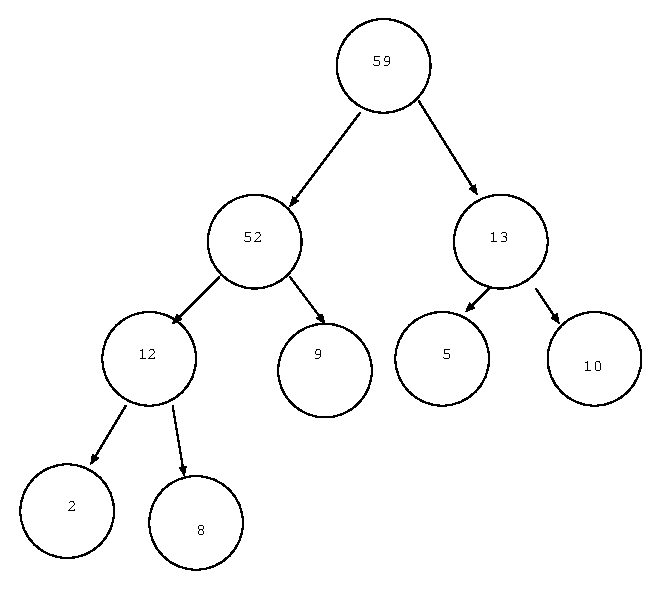
\includegraphics[scale=.7]{./maxheap.eps}
    \end{figure}

    $ \newline $

    First we will replace the removed element with the last element in the tree

    (b): 

    $ \newline $

    \begin{figure}[!htb]
        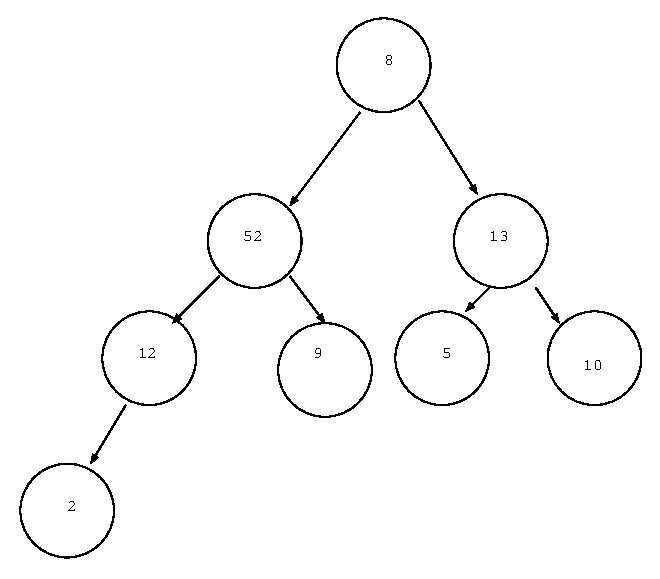
\includegraphics[scale=.7]{./removeHeap.eps}
    \end{figure}

    $ \newline $

    Then we must heapify the data structure

    \begin{figure}[!htb]
        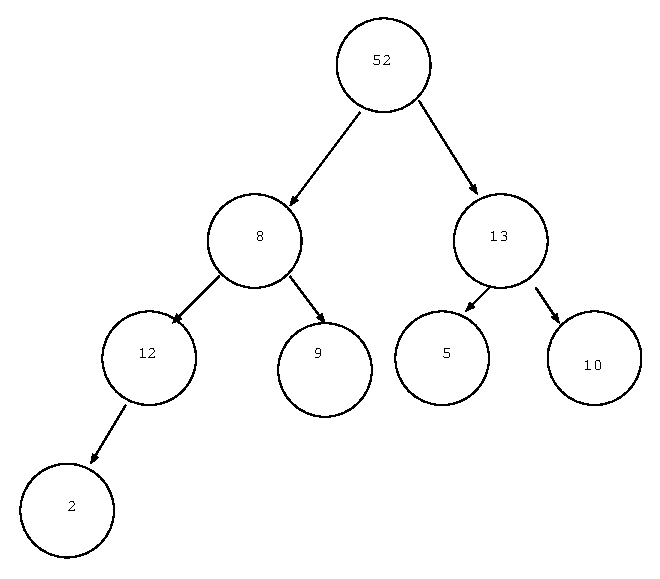
\includegraphics[scale=.7]{./removeMax2.eps}
    \end{figure}

    $ \newline $

    \begin{figure}[!htb]
        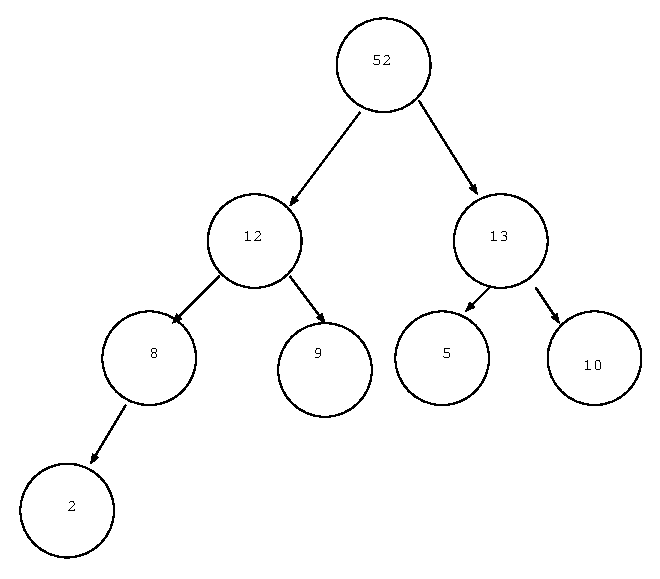
\includegraphics[scale=.7]{./removeMax3.eps}
    \end{figure}

    $ \newline $

    The max heap is now been heapified.

    $ \newline $

    2. Solve the following recurrences. You can not use master theorem to solve them. You must
    show the steps in your derivation.

    $ \newline $

    (a):  If we draw out a 3 iterations then we would get
    $ \newline $
    $ [cn]_{1} + [\frac{cn}{3} + \frac{2cn}{3}]_{2}]_{2} + [\frac{cn}{9} + \frac{2cn}{9} + \frac{2cn}{9} + \frac{4cn}{9}]_{3} $
    $ \newline $
    where the brackets represent the layers this can be reduced to $ [cn]_{1} + [cn]_{2} + [cn]_{3} + ... $ for all iterations.
    So now we just need to find the number of iterations. Every iteration divides n by 3 or by
    $ \frac{2}{3} $. This means that the tree wont be perfectly balanced. The tree will
    be its deapest on the right side of the tree because it will take more iterations for 
    it to equal 1. The right side of the tree will go for $ log_{3/2}(n) $ iterations. The left side of
    the tree will go for $ log_{3}(n) $ iterations. We will find the deepest path into 
    the tree so the value is $ log_{3/2}(n) * cn $.
    $ \newline $
    (b): First we will draw out a few iterations to find what the infinite series would be.
    $ \newline $
    The sum of the the function would be $ cn + \frac{cn}{5} + \frac{cn}{25} + ... $.
    $ \newline $
    Notice that the denominator $ 5^{i} $ where i is the iteration number. So we can write this
    as an infinite series. 
    $ \newline $
    $ \sum_{i=1}^{\infty} ( \frac{cn}{5} )^{i} $. 
    $ \newline $
    From this we can determine that the total sum is $ \frac{5nc}{4} $.
    $ \newline $
    (c): We will draw out the first few iterations again.
    $ [n^{log_{5}(7)}]_{0} + [\frac{n^{log_{5}(7)}}{2} + \frac{n^{log_{5}(7)}}{2}]_{1} + 
    [\frac{n^{log_{5}(7)}}{4} + \frac{n^{log_{5}(7)}}{2}]_{4} + \frac{n^{log_{5}(7)}}{2}]_{4} + 
    \frac{n^{log_{5}(7)}}{2}]_{4} ]_{2} + .... $
    $ \newline $
    As we can tell this can ben reduced to 
    $ n^{log_{5}(7)} + n^{log_{5}(7)} + n^{log_{5}(7)} + ... $ so that means 
    we just have to find the height of the tree. 
    $ \newline $
    Notice the denominator's value is $ 2^{i} $ where i is value of the iteration.
    So we know the last iteration is when $ \frac{n}{2^{i}} = 1 $ so there will be
    $ log_{2}(n) $ iterations. 
    So the sum is $ log_{2}(n) * n^{log_{5}(7)} $
    $ \newline $
    3. The worst case for this algorithm is that in the first comparison before the for loop
    the biggest element in the array is set to largest. In this case every
    the first comparison will fail and the second comparison will always be triggered. 
    the for loop will have $ (n - 2) $ iterations and two comparisons per iteration so
    inside the for loop there are $ 2(n - 2) $. The first comparison before the for loop
    will always be triggered so therefore in total there are $ 2n - 3 $ comparisons worst case.
    $ \newline $
    This algorithm will use divide and conqure strategy to divide the array into two sub arrays
    untill it only has 2 elements in the array. These arrays are then merged together where
    the first element is the largest element and the second in the array is the second largest
    element.
    $ \newline $
    \begin{verbatim}
        // start is the first index inclusive
        // finish is the last index inclusive
        // A is an array of elements
        function getGreatestAndSecondGreatestValue(A, start, finish) {
            T[] // T is an array of size 2
            if(finish - start == 1) {
                T[0] = max(A[start], A[finish])
                T[1] = min(A[start], A[finish])
                return T
            }

            Array1 = getGreatestAndSecondGreatestValue(A,start, start + floor((last-first)/2))
            Array2 = getGreatestAndSecondGreatestValue(A, start + ceil((last-first)/2), finish)
            merge(Array1, Array2)
        }

        // this merges two arrays keeping the greatest value on the left side of the new array and 
        // keeping the second greatest value on the right side of the array
        function merge(Array1, Array2) {
            MergedArray[] // array that will hold the merged results 
            MergedArray[0] = max(Array1[0], Array2[0])
            temp1 = max(Array1[1], Array2[0])
            temp2 = max(Array1[0], Array2[1])
            second = min(temp1, temp2)
            MergedArray[1] = second
            return MergedArray
        }

        function max(a,b) {
            return (a + b + abs(a - b)) / 2
        }

        function min(a,b) {
            ((a+b)-abs(a-b)/2)
        }

    \end{verbatim}

    There is a single comparitor used in every single node. We know that the height of the tree 
    is going to be $ \frac{n}{2} $ because the base case is 2. 
    $ \newline $
    T(n) = T(n/2) + 1
    $ \newline $
    We know that that the height of the tree is $ log_{2}(n) - 1 $ and there is a 
    sequence $ 2^{0} + 2^{1} + 2^{2} + ... + 2^{log_{2}(n)} $. $ \sum_{i=0}^{log_{2}(n) - 1}  $ = $ n - 1 $
    so this algorithm takes n - 1 comparisons.



    4. The k sorted list is assentialy several different sorted lists that occupy the same 
    memmory space. These lists just need to be merged in the order that they are in and then
    whatever is left needs to be inserted into the sorted sub array.

     \begin{verbatim}

     // A is the array 
     function sortKSorted(A, k, length) {
        range = length - k 
        if(k > range) {

        } else {

        }
        
        For i in range 
     }
     // N is Array given that needs to be sorted
     // I is the array of all the k sorted values
     // k is just keeping
     // i is the index 
     function mergeArrays(A[], I[], k, i, s) {

     }

     // this function stores elements that are not sorted
     function storeNonSorted(A[], from, to) {
        Temp[] // temporary array
        x = 0
        for(from in range(to)) {
            temp[x] = A[from]
        }
        return Temp
     }

     \end{verbatim}


    

    \end{document}

